\documentclass{article}
%\usepackage{fullpage}

\usepackage[english,french]{babel}
\usepackage[utf8]{inputenc}
\usepackage[T1]{fontenc}

\usepackage{amsmath, amsfonts, amssymb, amsthm}
\usepackage{bbm,algorithmic,algorithm,verbatim}

\usepackage{color}
\usepackage{subcaption}
\usepackage[pdftex]{graphicx}
\usepackage{epsfig}
\usepackage{ulem, stmaryrd, dsfont}
\usepackage{hyperref}

% \usepackage{mathabx} % for \vvvert ||| |||
\usepackage{./tex/sty/scribe}

%%%%%%%%%%%%%%%%%%%%%%%%%%%%%%%%%%%%%%%%%%%%%%%%%%%%%%%%%%%%%%%%%%%%%%%%%%%%%%%
% Hyperlinks
%%%%%%%%%%%%%%%%%%%%%%%%%%%%%%%%%%%%%%%%%%%%%%%%%%%%%%%%%%%%%%%%%%%%%%%%%%%%%%%

%\PassOptionsToPackage{hyphens}{url}
%\usepackage[pdftex,linkcolor=test,citecolor=vsomb_col,
%colorlinks=true,pagebackref,bookmarks=true,plainpages=true,
%urlcolor=fb_col]{hyperref}
\usepackage{cleveref}




\begin{document}
\sloppy
\lecture{HMMA308}{Lasso vs FoBa}{Tong Zhang}{Ophélie Coiffier}


%%%%%%%%%%%%%%%%%%%%%%%%%%%%%%%%%%%%%%%%%%%%%%%%%%%%%%%%%%%%%%%%%%%%%%%%%%%%%%%
%%%%%%%%%%%%%%%%%%%%%%%%%%%%%%%%%%%%%%%%%%%%%%%%%%%%%%%%%%%%%%%%%%%%%%%%%%%%%%%
In this report, we speak about three methods which predicted variables and with these predicted variables, we can compare the mean squared error on test and train values. For that, we use Lasso (using $L_1$ regularization), OMP ("Orthogonal Matching Pursuit", using forward greedy algorithm) and LARS (using forward and backward steps, such as FoBa (Forward-Backward) algorithm). Given that the FoBa function is available with the software R, we replace FoBa by LARS. But there is one significant difference : LARS tracks the path through $L_1$ penalized least squared error by gradually decreasing the regularization parameter and FoBa uses the insertion and deletion with unbiased least squared error. So, examples will not have the same results.\\
\begin{center}
    Which methods will be chosen to predict variables depending on the sparsity ?
\end{center}
First, we will describe our three methods then we apply them with real examples.
%%%%%%%%%%%%%%%%%%%%%%%%%%%%%%%%%%%%%%%%%%%%%%%%%%%%%%%%%%%%%%%%%%%%%%%%%%%%%%%
%%%%%%%%%%%%%%%%%%%%%%%%%%%%%%%%%%%%%%%%%%%%%%%%%%%%%%%%%%%%%%%%%%%%%%%%%%%%%%%


%%%%%%%%%%%%%%%%%%%%%%%%%%%%%%%%%%%%%%%%%%%%%%%%%%%%%%%%%%%%%%%%%%%%%%%%%%%%%%%
\section{Mathematic approach}
In this part, we will describe three methods to predict variables :
\begin{itemize}
    \item The Lasso 
    \item The OMP (Orthogoanl Matching Pursuit)
    \item The LARS (the closest equivalent for FoBa algorithm)
\end{itemize}

First, to measure the quality of prediction, we use a linear prediction model :
\[ f(x)=\trans{\beta}x\]
Where $\beta$ is a vector of coefficients, $x=(x_1, \cdots, x_n)$ the input variable ($x_i\in \R^d$ for i in $1$ to $n$) and $f(x)\approx y$ the output variable ($y=(y_1, \cdots, y_n$)).
Where $\beta$ is estimated by the empirical risk minimization : \[\hat{\beta}= \underset{\beta \in \R^d}\argmin \sum_{i=1}^n \Phi(\trans\beta x_i, y_i)\]
and $\Phi$ is loss function.\\
But $\hat{\beta}$ overfits the data so we need to adjust $\beta$. That's why, we obtain :
\[\hat{\beta} = \underset{\beta \in \R^d}{\argmin} \sum_{i=1}^n \Phi (\trans{\beta}x_i, y_i)+ \lambda g(\beta)\]
With $\lambda >0$ an adjustment parameter and $g(\beta)$ a regularization condition.

\subsection{The LASSO method}
The Lasso method uses the $L_1$ regularization. That means :
\[\hat{\beta} = \underset{\beta \in \R^d}{\argmin} \sum_{i=1}^n \Phi (\trans{\beta}x_i, y_i)+ \lambda ||\beta||_1\]
Where $||\beta||_1<k$ and $k$ is the sparsity parameter. Where $\lambda$ is a known regularization parameter and $\lambda>0$.\\
There are $2$ main issues with this method : 
\begin{itemize}
    \item Desirable feature selection property can only be achieve under relatively strong assumption.
    \item We need to use a large regularization parameter ($\lambda$) but it leads to sub-optimal prediction accuracy. To counteract this problem, we need a complex and less robust procedure.
\end{itemize}
\vspace{0.5cm}
An other method exists to predict variables and calculates its error (using loss function $\Phi$) : OMP method.

\subsection{The OMP method}
The second method that we will use in examples is the OMP method. It's a forward greedy algorithm. We use to improve an arbitrary prediction method or select relevant features. The principle is : add a feature at every step to aggressively reduce the squared error. But, like the previous method, there are issues and one of the most important is :
\begin{itemize}
    \item It never corrects mistakes made earlier steps. So it's inadequate for feature selection because it only works when small subsets of the basis functions are near orthogonal.
\end{itemize}
A solution is the backward greedy algorithm. The principle is to train a model with all the features and greedily remove one feature at a time. To choose the feature that we remove, we take these which have the smallest increase of squared error. Yet, if the number of features is higher than the number of samples, during the first step, $\beta$ overfits the data.\\
To counteract these problems, we can use a combination of both algorithms : forward and backward. It's the principle of FoBa method (and LARS method).

\subsection{The FoBa algorithm (method)}
This algorithm uses the Forward and Backward greedy algorithm. The approach that we use is : we want to use backward steps to remove any errors caused by earlier forward steps and to keep a reasonable number of basis functions. And we want to take backward step adaptively and make gain made in the forward steps. Actually, we use backward step when the squared error increase is no more than half of the squared error decrease in the earlier corresponding forward step. Moreover, it has a limited number of iterations so it is computationally efficient. \\
\\
\\
Now, we can compare these two principles methods : LASSO and FoBa.\\
The Lasso method allows to select features under some conditions. But we need to choose an appropriate non-zero threshold. And there are $2$ problems : the $L_1$ regularization parameter and the non-zero threshold (there are difficult to determine). Besides, we have a 'bias' with the $L_1$ regularization. While the FoBa method hasn't the same conditions to find the threshold parameter.\\
On the contrary, the FoBa greedy algorithm is closely related to the path-following algorithm for solving Lasso. The LARS algorithm (a closer algorithm of FoBa) starts with a large regularization parameter such as Lasso, then it is gradually decreased. We can remind us that LARS tracks the path through $L_1$ penalised least squared error by gradually decreasing the regularization parameter. But this way to find regularization parameter produces a significant bias. That is a difference between LARS and FoBa because FoBa which tracks the insertion and deletion with unbiased least squared error. It will be needed to wait a few iterations to reduce the regularization parameter and finally reduce the bias to look like the FoBa parameter. Last, Lasso and FoBa has an other similarity : mistakes made in earlier steps can be removed later. That is not possible with a forward greedy algorithm (an OMP method).\\

In the next part, we will compare these three methods with two examples : one with \textit{Ionosphere} data, one with \textit{Boston Housing} data.

%%%%%%%%%%%%%%%%%%%%%%%%%%%%%%%%%%%%%%%%%%%%%%%%%%%%%%%%%%%%%%%%%%%%%%%%%%%%%%%

%%%%%%%%%%%%%%%%%%%%%%%%%%%%%%%%%%%%%%%%%%%%%%%%%%%%%%%%%%%%%%%%%%%%%%%%%%%%%%%
\section{Examples with comparison of three methods}
In the second part, we will use the mean squared error as loss function. It is equivalent to :
 \[MSE = \frac{1}{n} \sum_{i=1}^n (\hat{Y}_i-Y_i)^2\]
 Where $\hat{Y}$ is the vector of predicted values and $Y$ the vector of obseved values. Where $n$ is the dimension of $Y$.\\
 We remind us that $Y$ is the vector of the desired output.\\
 Then, we will predict variables thanks to the randomly partition into $50$ training points and $test\_size$ (defined for each example) test points. Finally, we will compare the mean squared error for each methods and for each groups (test and training points).\\
 Data is available on websites : \href{https://archive.ics.uci.edu/ml/machine-learning-databases/housing/}{https://archive.ics.uci.edu/ml/machine-learning-databases/housing/}\cite{house} and \href{https://archive.ics.uci.edu/ml/datasets/ionosphere}{https://archive.ics.uci.edu/ml/datasets/ionosphere}\cite{iono}. \\
 And Python code is available on the Github \cite{code}.

%%%%%%%%%%%%%%%%%%%%%%%%%%%%%%%%%%%%%%%%%%%%%%%%%%%%%%%%%%%%%%%%
\subsection{First example : Boston Housing data}
\subsection{First example : Boston Housing data}
\textit{Boston housing} data is $506$ census tracts of Boston from the $1970$ census. So we have $506$ data-points (for each census) and $14$ features. Actually, we have $13$ different features and a $14th$ feature corresponding with a constant offset one. The desired output is the housing price (the $y$ vector in  the mathematics approach).\\
As we explain before this subsection, we partition the data points into $2$ groups : training points and test points. We have $50$ training points and $456$ test points. We calculate the average squared error (MSE) between the predicted values of $y$ and the true values. We repeat this, $50$ times and we calculate the mean of these MSE. We do this for the three methods : Lasso, Lars and OMP. Moreover, we use a sparsity starting at $1$ and stopping at $10$. We obtain these graphs (Figure $1$ $\&$ Figure $2$).
\begin{figure}[!ht]
    \centering
    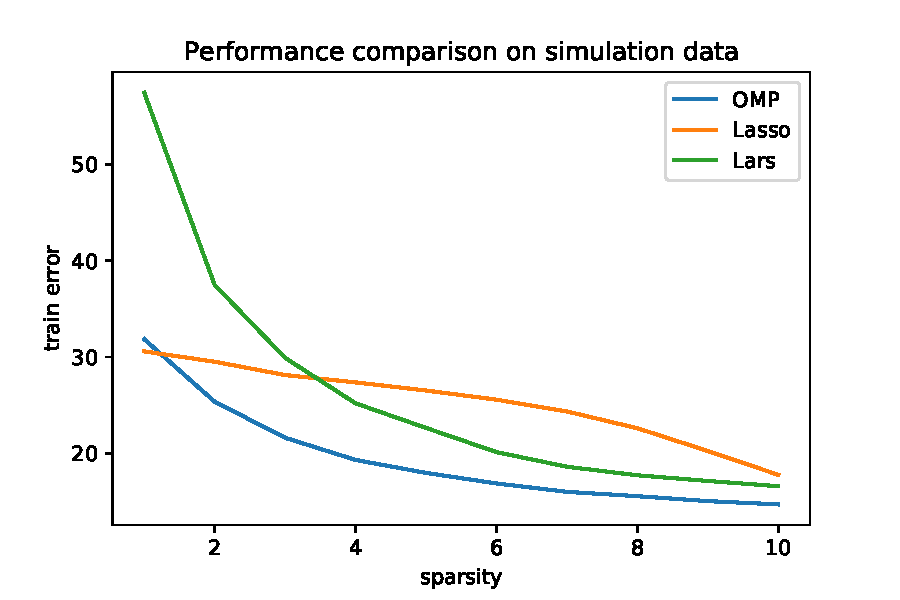
\includegraphics[scale=0.5]{./images/training_error_housing.pdf}
    \caption{MSE comparison on training points with Boston housing's data}
    \label{Figure 1}
\end{figure}
The better method has a smaller MSE than others.\\
This graph shows us that the OMP method has a better prediction than the Lars method, which has a better prediction than the Lasso method. Besides, all the curves decrease : they begin between $59$ and $30$ and they achieve $15-20$.\\
The problem is : we don't have the same figure than the article. The curves behavior is the same but in the main article, the three curves begin to $59$ and finish to $10-15$. Maybe the cause is : we don't use the same method (the main article uses FoBa algorithm, Forward-greedy algorithm and backward algorithm). Actually, we choose a specific method using these algorithms not basic algorithms. On the main article graph, we find that FoBa algorithm is better than backward and backward is better than forward : the opposite of our finding.\\
\\
Let's compare the test points (Figure $2$).\\
\begin{figure}[!ht]
    \centering
    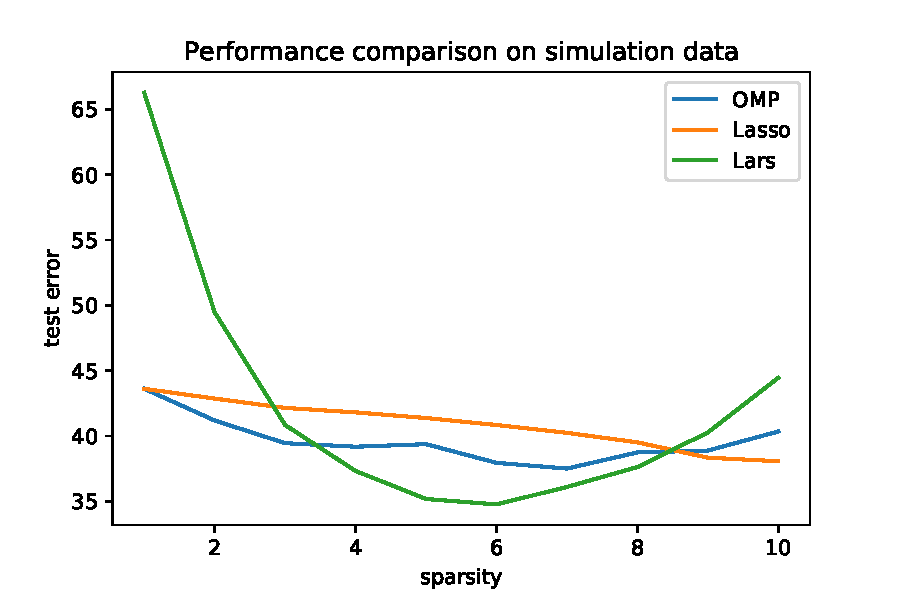
\includegraphics[scale=0.5]{./images/test_error_housing.pdf}
    \caption{MSE comparison on test points with Boston housing's data}
    \label{Figure 2}
\end{figure}
Once more, we don't have the same graph than the main article. Here, we choose the Lars method when the sparsity is superior at $3$ and inferior at $9$. Before, we choose the OMP method and after, we choose the Lasso method. We can observe that the Lars curve decreases (start : $45$, stop : $35$) until it achieves a sparsity of $6$ then it increases (between $35$ and $45$). The OMP curve decreases until it achieves a sparsity of $7$ (start : $43$, stop : $37$), then it lightly increases (between $37$ and $41$). And the Lasso curve gradually decreases between $44$ and $38$.\\
In the main article the three curves decrease between $60-63$ and $35$ for a sparsity included in $1$ and $5$. The better method is FoBa, then backward and finally forward algorithm. Between a sparsity of $5$ and $10$ they increase (start : $35$, stop : $40-44$) and the better method becomes backward algorithm (followed by forward algorithm). Finally, FoBa becomes the worst method. Actually, if we begin our representation at the sparsity of $3$, we obtain the same best method until a sparsity of $10$.
\\
Now, we will apply the mathematics approach with \textit{Ionosphere} data.

%%%%%%%%%%%%%%%%%%%%%%%%%%%%%%%%%%%%%%%%%%%%%%%%%%%%%%%%%%%%%%%%%
\subsection{Second example : Ionosphere data}
\textit{Ionosphere} data contains $351$ data points with $35$ features. As the other data set, the $35th$ feature is a constant offset one. The $y$ vector corresponds to a binary valued : $0$ or $1$. It's the desired output.\\
As we explain in the introduction of this part, we partition the data points into $2$ groups : training points and test points. We have $50$ training points and $301$ test points. As the previous data, we calculate the mean squared error (MSE) between the predicted values of y and the true values. We repeat this, $50$ times and we calculate the average of these MSE. We realise this with the three methods : Lasso, Lars and OMP. Moreover, we use the same sparsity than the other data set : between $1$ and $10$. Results are represented in Figure $3$ and Figure $4$.\\
\\
\begin{figure}[!ht]
    \centering
    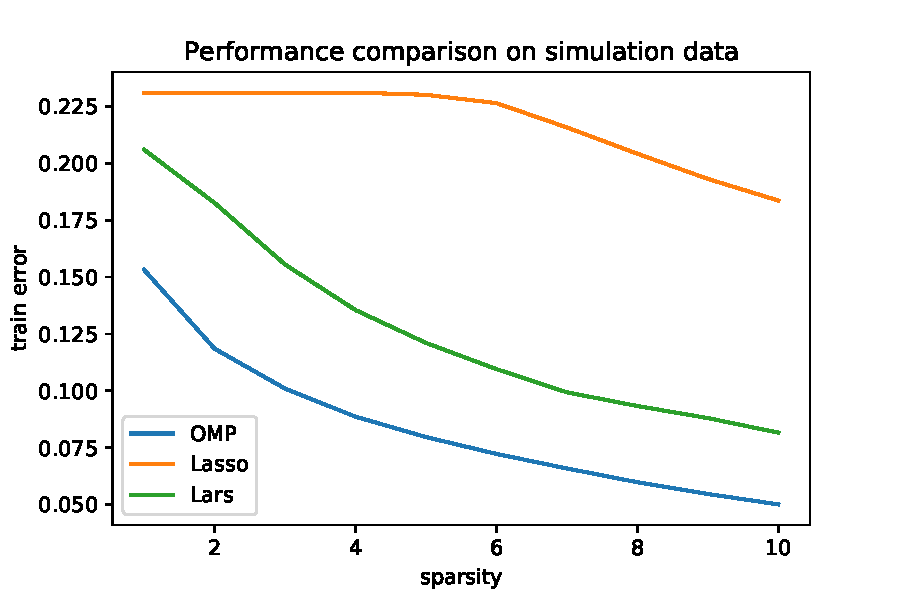
\includegraphics[scale=0.5]{./images/training_error_ionosphere.pdf}
    \caption{MSE comparison on training points with Ionosphere's data}
    \label{Figure 3}
\end{figure}
We observe in this figure (Figure $3$) that OMP and Lars curve decrease with the same "shape" while Lasso curve decreases from a sparsity of $4$ and stagnates between a sparsity of $1$ to $5$. The OMP curve decreases between $0.150$ and $0.05$ while Lars curve decreases between $0.20$ and $0.075$. The Lasso curve stagnates at $0.225$ between a sparsity of $1$ and $5$, then it decreases from $0.225$ to $0.03$. So, we choose the method which have the smallest error : the OMP method until a sparsity of $8$, then we take the Lasso method.\\
Our problem stays the difference between our representation and these of the main article. In this article, the three curves decrease and the better method is FoBa algorithm. All curves decrease between $0.17$ and $0.05-0.07$. The ranking of the best algorithm is : FoBa, forward-greedy then $L_1$. Our ranking was : OMP (forward-greedy algorithm), FoBa then Lasso ($L_1$).\\
\\
\begin{figure}[!ht]
    \centering
    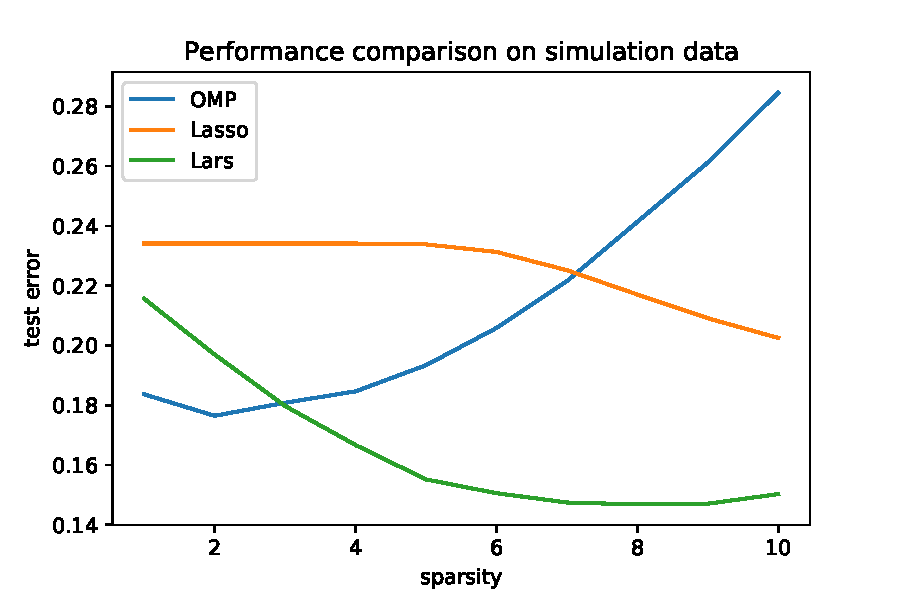
\includegraphics[scale=0.5]{./images/test_error_ionosphere.pdf}
    \caption{MSE comparison on test points with Ionosphere's data}
    \label{Figure 4}
\end{figure}
Let's compare the test points (Figure $4$).\\
Thanks to this representation, we choose the Lars method when the sparsity is superior to $3$. When the sparsity is inferior to $3$, we choose OMP method. The worst method stays the Lasso method until a sparsity of $3$, then it becomes OMP method. The Lasso curve stagnates at $0.235$ between a sparsity of $1$ and $4$, then it decreases (start : $0.235$, stop : $0.17$) and finally, the curve increases until $0.24$. While Lars curve decreases between $0.22$ and $0.15$ until a sparsity of $7$ then it lightly increases. The OMP decreases until a sparsity of $2$ (start : $0.19$, stop : $0.17$), then it increases between $0.17$ and $0.30$.\\
Once more, it isn't the same result than the main article. In this article, the best algorithm is $L_1$ (for each sparsity) and the worst is  FoBa algorithm. Moreover, the $L_1$ curve decreases between a sparsity of $1$ and $3$, then it increases. The two others gradually increase.\\ 

%%%%%%%%%%%%%%%%%%%%%%%%%%%%%%%%%%%%%%%%%%%%%%%%%%%%%%%%%%%%%%%%%%%%%%
\subsection{Our issues}
All of our representations are different to the representations of the Tong Zhang's article. An explanation will be the method used : we use function like OMP, Lasso and Lars to represent FoBa, $L_1$ and forward greedy algorithms. Or/And the $\lambda$ coefficient to implement Lasso function. But our choices of the best method is the opposite of his algorithm choice. So, I don't think it's the only issue that we have....\\
Generally, we have the same "shape" of curves and the same order of magnitude. It's the only positive point that we have....
We have an issue about the scale of Lasso curve too : \\
To find the Lasso coefficient, we use the function \textit{Lasso\_path}.
\begin{itemize}
    \item \textit{Boston housing} data\\
The figure $5$ shows us how we choose the alpha coefficient in Lasso method.
\begin{figure}[!ht]
    \centering
    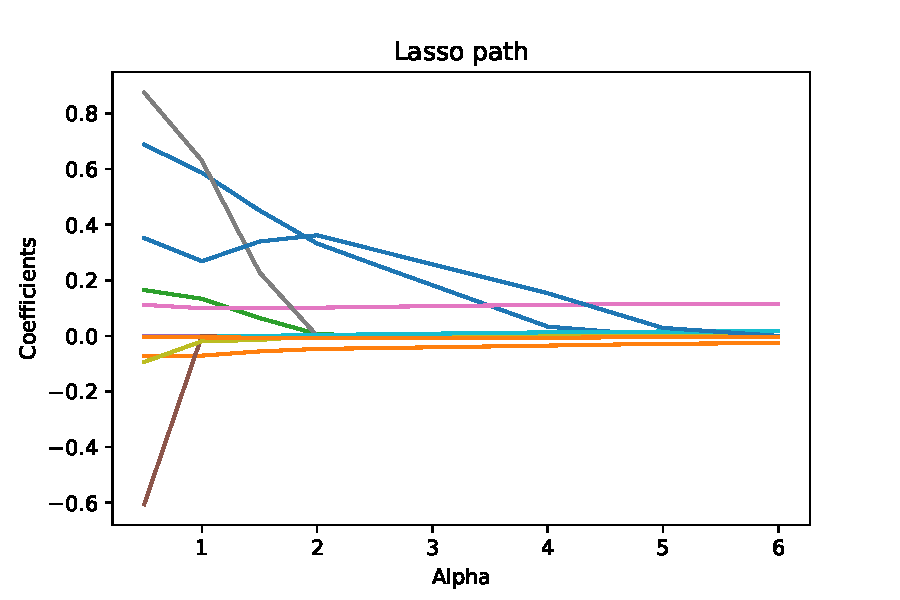
\includegraphics[scale=0.6]{./images/alpha_choice_lasso_house.pdf}
    \caption{Number of coefficients which are different of $0$ depending on alpha coefficient.}
\end{figure}
Each lines different to $0$ correspond to a non zero coefficient for the explanatory variable. For example, if we take $alpha=6$, we have one non zero coefficient. If we have $alpha=3$, we have $4$ non-zero coefficients. We have created an array of different alpha coefficients. We test some values and we stop to this array : $[0.5, 1.0, 1.5, 2.0, 2.5, 3.0, 3.5, 4.0, 5.0, 6.0]$. The figure $6$ shows us the number of non zero coefficient depending on alpha coefficient.
\begin{figure}[!ht]
    \centering
    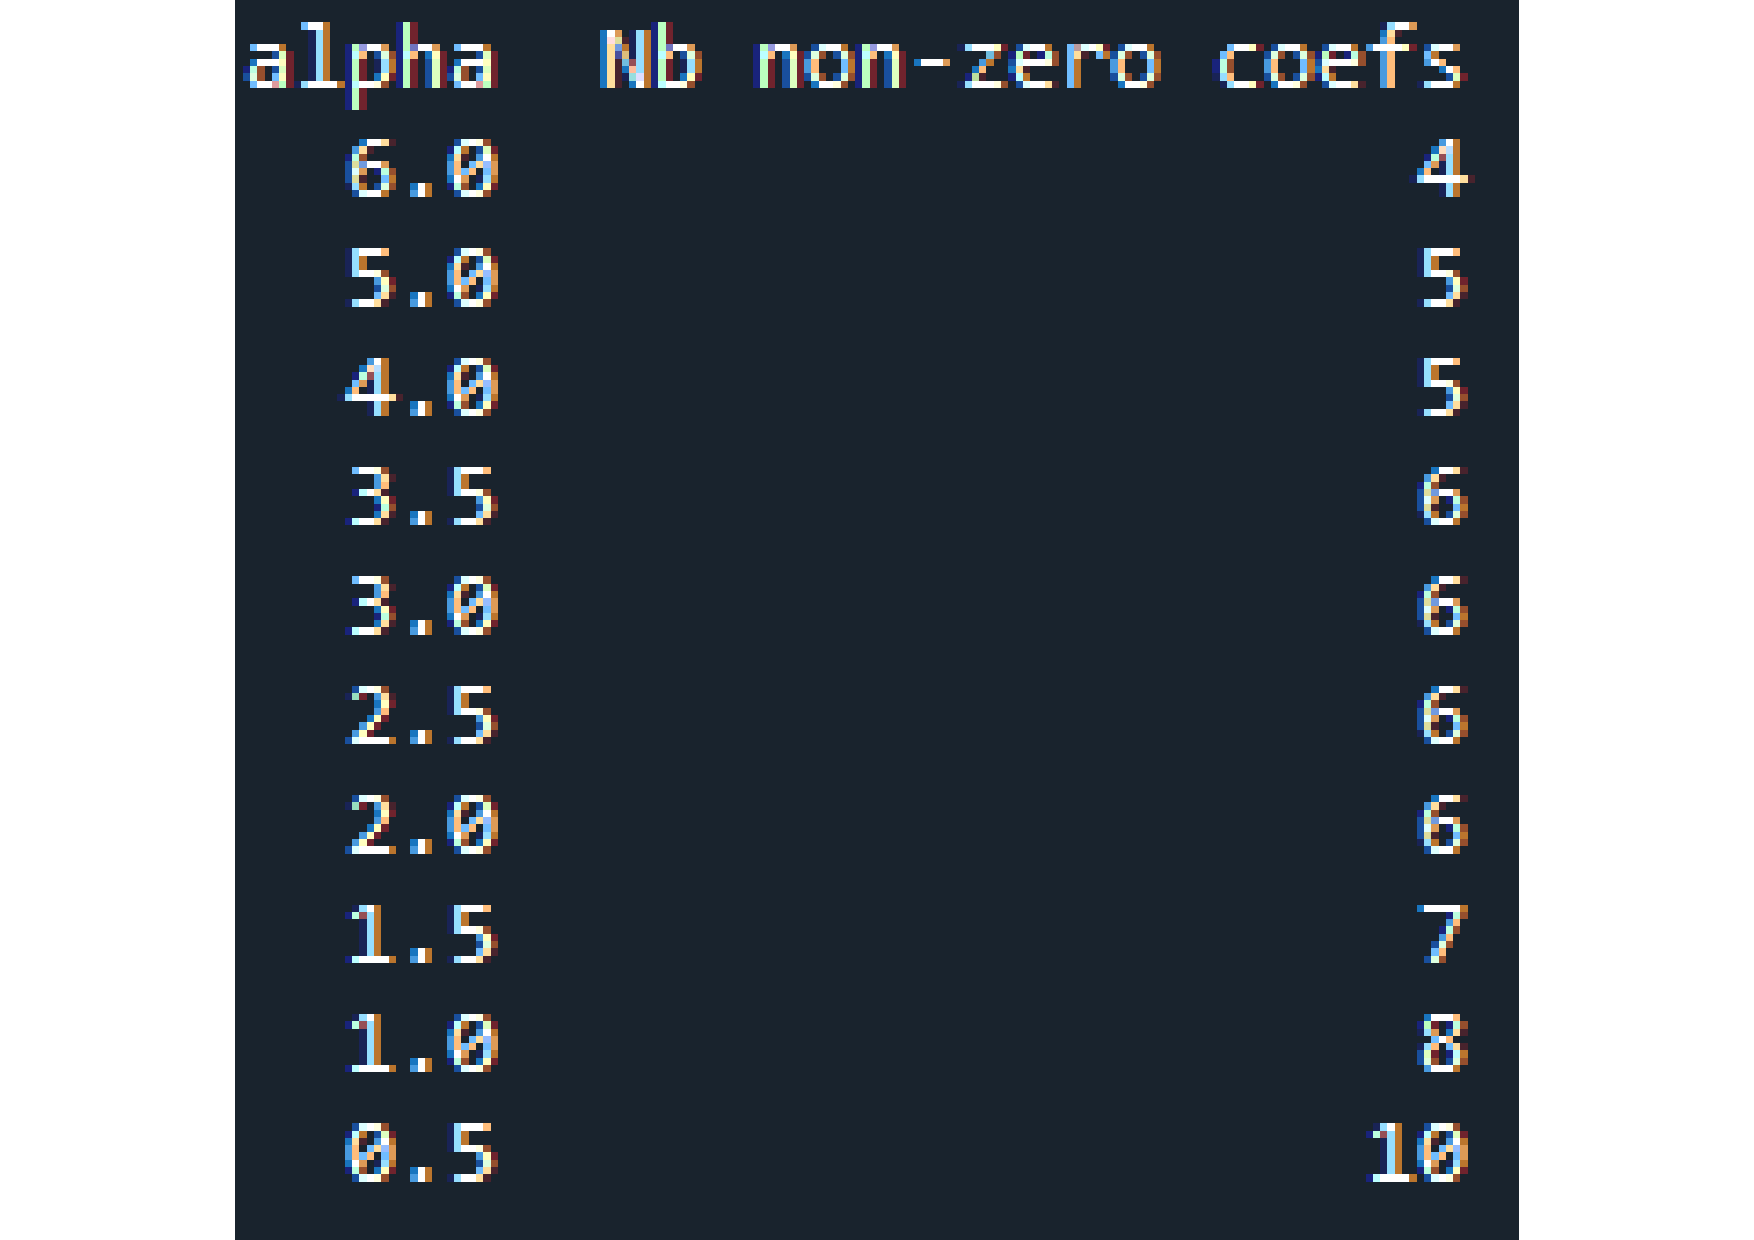
\includegraphics[scale=0.2]{./images/nb_non_zero_house.pdf}
    \caption{Number of coefficients which are different of $0$ depending on alpha coefficient.}
\end{figure}
The problem is : we have the same coefficient several times and the order of these numbers are not the same that we use to represent the MSE depending on sparsity. So, we can't have the good scale to compare MSE with the other method. The two other method has a growing number of non zero coefficient, it is not stagnant like the Lasso method. Moreover, the list of non zero coefficient number is different to $[1, 2, 3, 4, 5, 6, 7, 8, 9 ,10]$ because we have $[4, 4, 6, 6, 6, 6, 7, 9, 10, 11]$. I don't manage to create this type of list with alpha coefficients. It is one of our issues.
\\
   \item \textit{Ionosphere} data\\
We use the same method than \textit{Boston housing} data to create sparsity in Lasso method. So we meet the same issue.\\
The Figure $7$ shows us the representation of Lasso path using the alpha array : $[0.004,0.006,0.01,0.05,0.1,0.15, 0.2, 0.25, 0.3, 0.4]$.\\
   \begin{figure}[!ht]
    \centering
    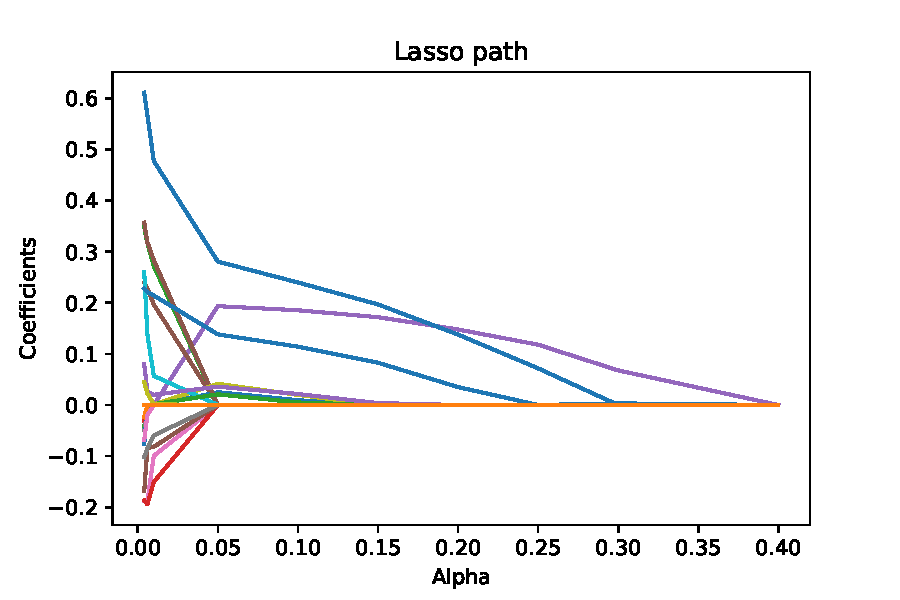
\includegraphics[scale=0.6]{./images/alpha_choice_lasso.pdf}
    \caption{Number of coefficients which are different of $0$ depending on alpha coefficient.}
\end{figure}
The figure $8$ represents the number of non zero coefficients depending on alpha coefficients. We find some number several times. We have the same problem too.
\begin{figure}[!ht]
    \centering
    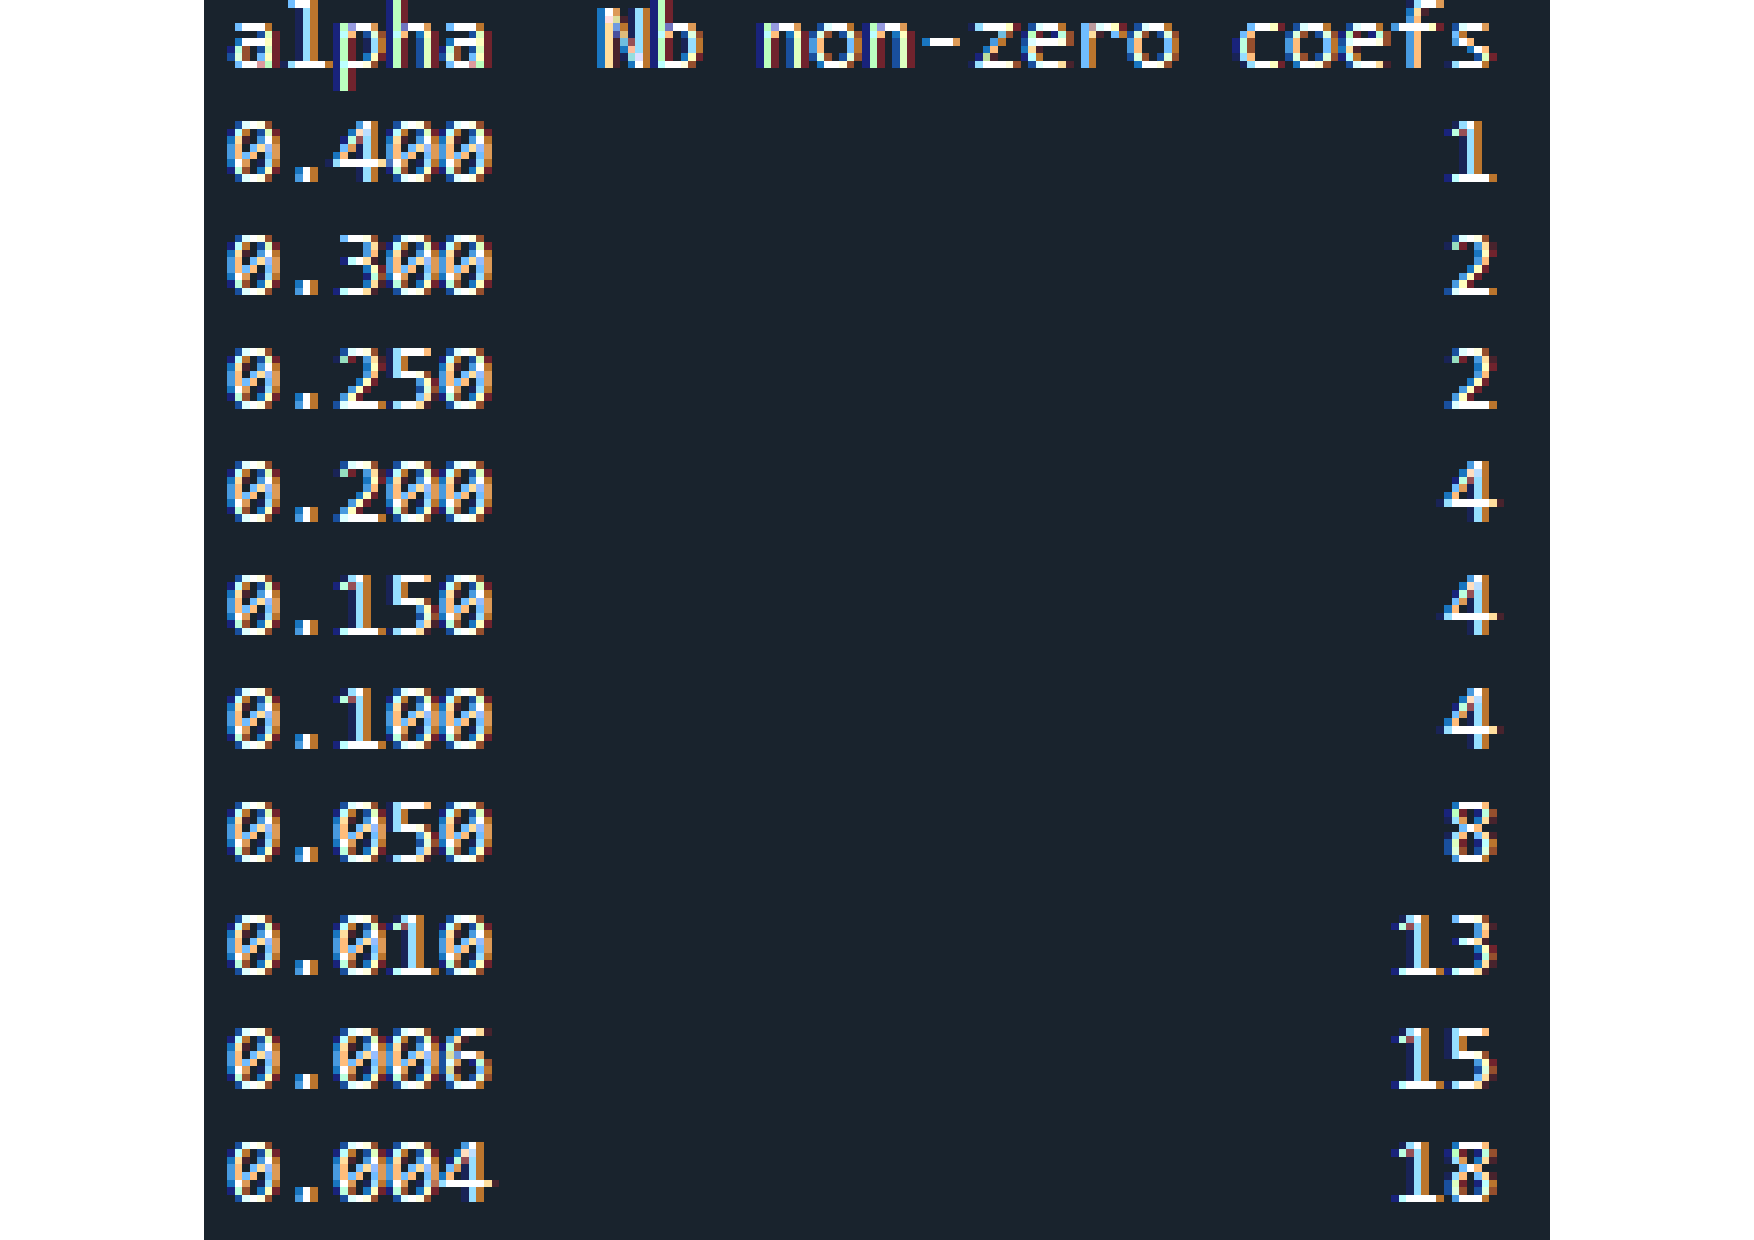
\includegraphics[scale=0.2]{./images/nb_non_zero_ionosphere.pdf}
    \caption{Number of coefficients which are different of $0$ depending on alpha coefficient.}
\end{figure}
\end{itemize}
We find one of our issues but I don't manage to avoid it.....
\newpage

%%%%%%%%%%%%%%%%%%%%%%%%%%%%%%%%%%%%%%%%%%%%%%%%%%%%%%%%%%%%%%%%%%%%%%%

%%%%%%%%%%%%%%%%%%%%%%%%%%%%%%%%%%%%%%%%%%%%%%%%%%%%%%%%%%%%%%%%%%%%%%%
\section*{Conclusion}
The main question is about the learning sparse representations using greedy algorithms.\\
We find these results :\\
For test points, FoBa algorithm (represented by Lars method) is the best algorithm with \textit{Ionosphere} data and it's FoBa or OMP (depending on sparcity) with \textit{Boston housing} data. That means it's the algorithm which predicts $y$ with less mistakes. We remind us that we use Mean Squared Error (MSE) and we could use an other loss function to check our findings.\\
For training points, we find OMP method (forward-greedy algorithm) for both data sets. With \textit{Ionosphere} data we need to have a small sparsity to keep the OMP method. If we have a large sparsity, we choose Lasso method ($L_1$ regularization).\\
\\
Actually, according to the article, only the mixed algorithm : FoBa is useful with training points. We need to use a novel combination of the forward-greedy and backward-greedy algorithms to obtain a smaller error. For test points and \textit{Boston housing} data, better sparsity leads to a change of the useful algorithm. And with \textit{Ionosphere} data, the $L_1$ regularization leads to better performance : the "bias" helps to have a sub-optimal sparsity. In other words, it is an advantageous with these points and data. \\
\\
Finally, we must choose the best algorithm and the best method depending on data, sparsity and mathematics conditions that we can check.


%%%%%%%%%%%%%%%%%%%%%%%%%%%%%%%%%%%%%%%%%%%%%%%%%%%%%%%%%%%%%%%%%%%%%%%%%%%%%%%

%%%%%%%%%%%%%%%%%%%%%%%%%%%%%%%%%%%%%%%%%%%%%%%%%%%%%%%%%%%%%%%%%%%%%%%%%%%%%%%
%%%%%%%%%%%%%%%%%%%%%%%%%%%%%%%%%%%%%%%%%%%%%%%%%%%%%%%%%%%%%%%%%%%%%%%%%%%%%%%
\section{Deal with linear models in depth}
\label{sec:pour_aller_plus_loin_sur_ce_theme}
%%%%%%%%%%%%%%%%%%%%%%%%%%%%%%%%%%%%%%%%%%%%%%%%%%%%%%%%%%%%%%%%%%%%%%%%%%%%%%%
%%%%%%%%%%%%%%%%%%%%%%%%%%%%%%%%%%%%%%%%%%%%%%%%%%%%%%%%%%%%%%%%%%%%%%%%%%%%%%%

We can read the article and the lesson to learn more about the Machine Learning and the Adaptive FoBa algorithm :
\cite{Article}, \cite{Teaching}\\
To visualize the Python code, we can go to the Github :
\cite{code} and go to the sklearn website to visualize functions used : \cite{algo} 

\newpage
%%%%%%%%%%%%%%%%%%%%%%%%%%%%%%%%%%%%%%%%%%%%%%%%%%%%%%%%%%%%%%%%%%%%%%%%%%%%%%%
\bibliographystyle{alpha}
\bibliography{./tex/biblio/references}
%%%%%%%%%%%%%%%%%%%%%%%%%%%%%%%%%%%%%%%%%%%%%%%%%%%%%%%%%%%%%%%%%%%%%%%%%%%%%%%


\end{document}